\begin{figure*}[t]
\centering
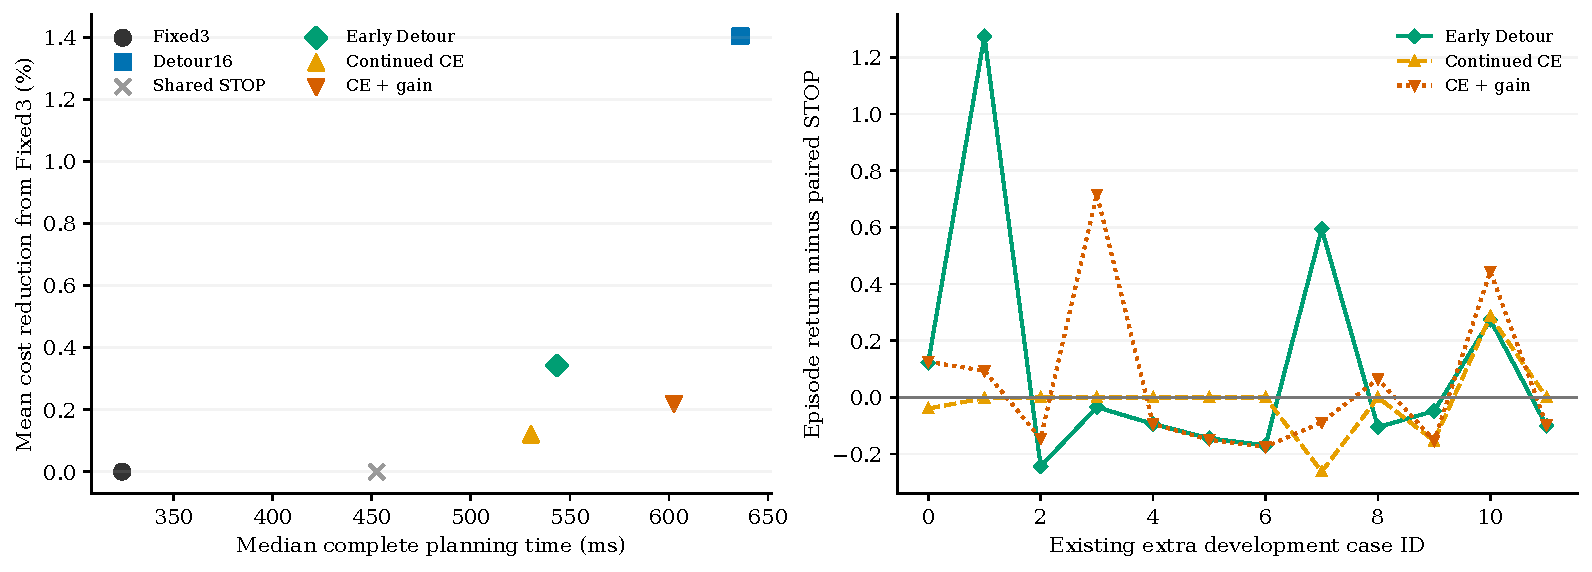
\includegraphics[width=0.95\textwidth]{figures/quality_time_returns.pdf}
\caption{Frozen-policy feedback on 12 previously used development scenes (four regular, four mixed and four blocked). Left: mean per-scene cost reduction in $J=L+0.75K$ versus median resident-model complete planning time, including fresh scene preparation and final proxy validation. Right: paired shared-environment returns relative to immediate STOP; original Fixed3 and Detour have no comparable shared-work return and are omitted from that panel. All 72 scene-method plans are single timing observations. Model loading is separate and instrumentation overhead is included; these points do not establish a stable time advantage or generalization. Detour16 uses its original action space, whereas the four shared methods use the G2 menu. No weights were updated and no PPO was run.}
\label{fig:g22_performance}
\end{figure*}
\begin{figure*}[t]
\centering
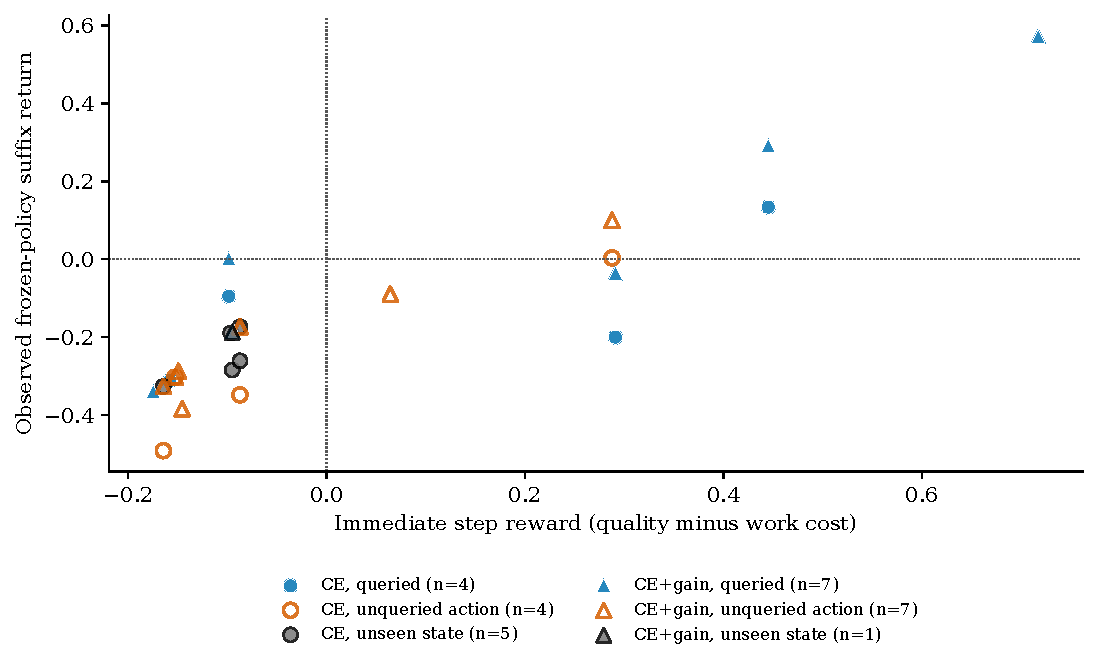
\includegraphics[width=0.95\textwidth]{figures/action_outcomes.pdf}
\caption{The 28 actual non-STOP proposals from the two frozen models. Points distinguish an action queried at the exact saved teacher state, an unqueried action at a saved state, and a state absent from that teacher. Immediate reward and the actual remaining return under the frozen policy are different observations. The suffix includes future actions and terminal validation corrections; it is neither optimal $Q$ nor the original depth-2 teacher target. A negative suffix can still outperform STOP, which also incurs pending menu cost; the horizontal zero line is not a STOP advantage boundary. Points from the same episode are correlated. Unknown actions can help or hurt and receive no imputed negative label.}
\label{fig:g22_actions}
\end{figure*}
